\section{Datos y análisis exploratorio}
\subsection{Fuente de datos}
Se utilizó la Encuesta de Hogares (EH) 2025 del Instituto Nacional de Estadística (INE) de Bolivia, tablas de Persona, Vivienda, Equipamiento y Seguridad Alimentaria (catálogo ANDA). Las estimaciones poblacionales usan el factor de expansión muestral del INE. La unidad de análisis es el hogar: una fila por identificador \texttt{folio} (formato UPM-segmento-persona; los dos primeros bloques identifican el grupo de muestreo).

\subsection{Construcción de la base de hogares}
Las cuatro tablas comparten exactamente los mismos 12.726 hogares, por lo que la unión por \texttt{folio} no produjo pérdidas. A partir de la tabla Persona se agregaron variables del hogar: tamaño, número y proporción de menores de 14 años y adultos mayores, miembros ocupados, tasa de dependencia, promedio de años de estudio de los miembros de 15 años o más, y tipología de hogar. Del jefe/a de hogar (identificado con la variable de parentesco del INE, exactamente uno por hogar) se tomaron sexo, edad, nivel y años de estudio, condición de actividad, tipo y grupo de ocupación. De Vivienda se conservaron las características de la vivienda y se construyeron los dormitorios, las personas por dormitorio y el hacinamiento (>2,5 personas por dormitorio). De Seguridad Alimentaria se construyó el puntaje FIES (0--8) y su nivel (segura, leve, moderada, severa). De Equipamiento se pivotaron los 18 bienes durables a una fila por hogar más el total de activos.

\subsection{Limpieza y hogares excluidos}
Todas las decisiones de limpieza están documentadas en \texttt{decisiones\_limpieza.md}. Las principales: los códigos de ``no aplica'' se trataron como categoría propia y no como faltantes (p.~ej. jefe sin ocupación, 2.146 hogares); los dormitorios reportados en cero se imputaron a uno (1.046 hogares); las preguntas FIES sin respuesta se contaron como negativas; y los nulos de servicios que no aplican (desagüe, baño compartido, tipo de internet) se codificaron como 0. \textbf{No se excluyó ningún hogar}: las cuatro tablas contienen los mismos 12.726 folios. Las tablas de gastos alimentarios y no alimentarios del INE no se utilizaron por ser proxies del ingreso (riesgo de fuga de datos).

\subsection{Variable objetivo y prevención de fuga de datos}
La variable objetivo principal es \texttt{p0}, la condición de pobreza por ingreso calculada por el INE (ingreso per cápita del hogar frente a la línea de pobreza). \texttt{pext0} (pobreza extrema) se usa solo como etiqueta secundaria y no entra al modelo, pues deriva del mismo ingreso. El factor de expansión se usa exclusivamente para estadísticas ponderadas y nunca como predictor. Se verificó que ningún predictor proviene del ingreso: existe una lista negra explícita de 99 variables de ingreso/gasto del módulo de persona.

\subsection{Análisis exploratorio}
La pobreza por ingreso alcanza al 37,8\,\% de los hogares (ponderada; 37,9\,\% sin ponderar) y la pobreza extrema al 13,9\,\% ponderada. El desbalance es moderado. La Tabla~\ref{tab:pobreza_area} muestra la pobreza por área y la Figura~\ref{fig:pobreza_depto} la variación por departamento.

\begin{table}[ht]\centering\caption{Pobreza ponderada por área (EH 2025).}\label{tab:pobreza_area}
\begin{tabular}{lrr}\toprule Área & Hogares (muestra) & Pobreza (\%) \\\midrule
Urbano & 9.611 & 31,8 \\
Rural & 3.115 & 50,9 \\\bottomrule\end{tabular}\end{table}

La pobreza es sustancialmente mayor en el área rural (50,9\,\%) que en la urbana (31,8\,\%). Por departamento, Potosí registra la mayor tasa (50,1\,\%) y Santa Cruz la menor (25,9\,\%); Cochabamba (37,1\,\%, $n$=2.198) se ubica ligeramente por debajo del promedio nacional. Entre los factores asociados destacan la educación del jefe/a (59,6\,\% de pobreza sin estudios frente a 15,8\,\% con 16 o más años), el hacinamiento (60,1\,\% frente a 32,6\,\%) y el equipamiento del hogar (52,4\,\% con 0--4 bienes frente a 5,3\% con 13--18). La inseguridad alimentaria se asocia con mayor pobreza (53,1\,\% en nivel moderado frente a 29,5\,\% en hogares con seguridad alimentaria), aunque puede ser consecuencia y no causa.

\begin{figure}[ht]\centering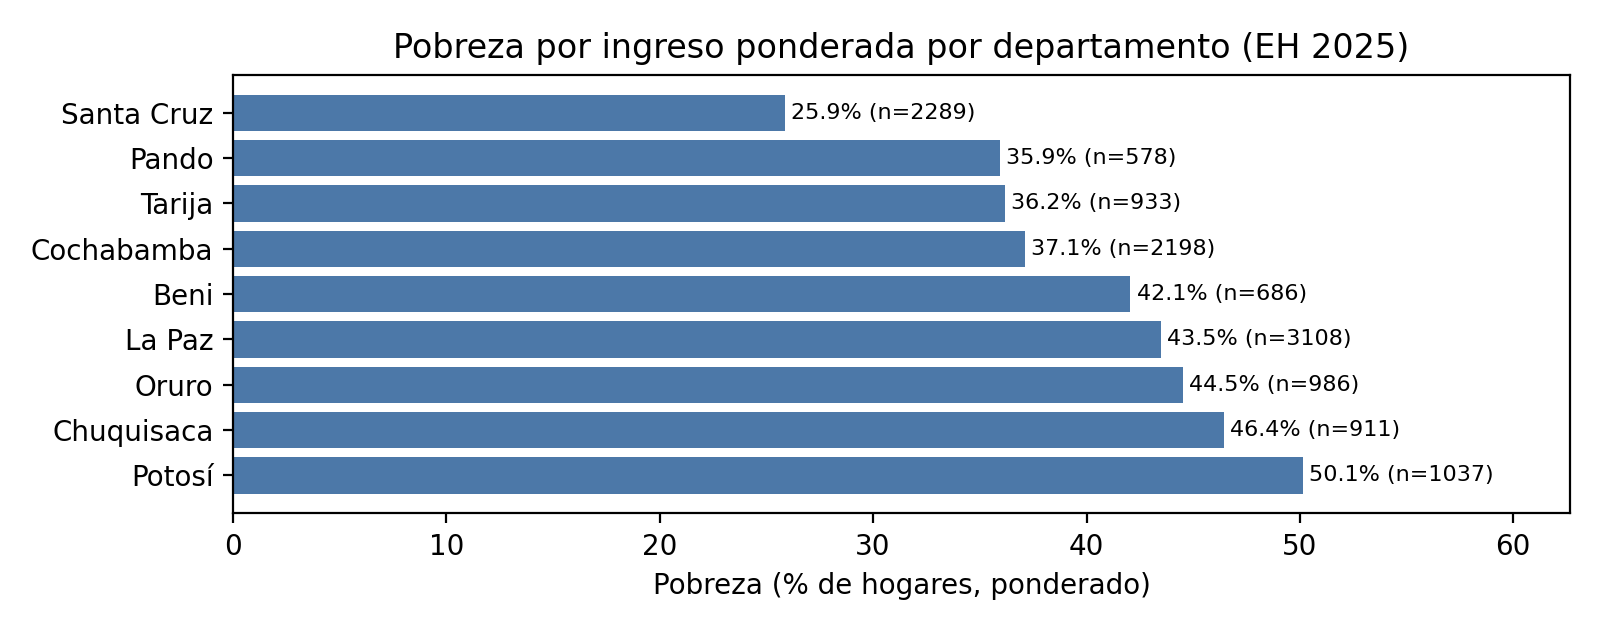
\includegraphics[width=.8\textwidth]{figuras/eda_01_pobreza_depto.png}
\caption{Pobreza ponderada por departamento (EH 2025).}\label{fig:pobreza_depto}\end{figure}

\subsection{Limitaciones}
La etiqueta de pobreza es monetaria (ingreso per cápita frente a la línea de pobreza), por lo que está sujeta a subdeclaración del ingreso. Los datos son transversales: las asociaciones encontradas no implican causalidad. La inseguridad alimentaria puede ser consecuencia de la pobreza más que causa. Finalmente, la muestra es una encuesta por muestreo: las tasas no ponderadas describen a los hogares encuestados, no a la población.
